\documentclass[]{msulabm}
\usepackage[utf8]{inputenc}
\usepackage{amsmath}
\usepackage{graphicx}
%\usepackage[linktocpage]{hyperref}  % if not using colorlinks, use linktocpage
\usepackage[colorlinks]{hyperref}  % if not using colorlinks, use linktocpage
\usepackage{bm}            % bold math
\usepackage{multirow}
\usepackage[table]{xcolor} % provide alternating rows with colors
\usepackage{textcomp}
\usepackage{xfrac} % gives split-level fractions with '\sfrac{a}{b}
\usepackage{multicol}
\usepackage[section]{placeins} % provides \FloatBarrier, to keep floats from crossing this barrier
\usepackage{amssymb}
\usepackage{wrapfig} % provides wrapping figures with text.
%\usepackage{enumitem} % gives \begin{enumerate}[resume] to resume counting from previous enumerate
%\usepackage{subfigure}
%\usepackage{tikz} % to draw arrows
\usepackage{xtab} % provides xtabular, tabular environment that spans multiple pages and other awesome things
\usepackage[style=phys,biblabel=brackets,pageranges=false]{biblatex}
\usepackage{pdflscape}
\usepackage{ragged2e}
\usepackage{longtable}
\usepackage{mathabx} % gives astronomy symbols like \Earth
\usepackage{pdfpages}

\bibliography{references-manual,bbarker-zotero}

\newcommand{\abs}[1]{\left\lvert#1\right\rvert}

\title{Laboratory Manual}
\author{ASTR 24100 Physics of Stars \\ \\ The University of Chicago}
\date{Winter 2019}

\pagestyle{ruled}

\definecolor{lgray}{rgb}{.2,.2,.2}

\makeevenfoot{ruled}{\thepage}{\footnotesize{\textit{Last updated \today}}}{}
%\makeevenfoot{ruled}{\thepage}{}}{}
\makeoddfoot{ruled}{}{\color{lgray} \tiny{This work is licensed under \href{http://creativecommons.org/licenses/by-sa/4.0/}{CC BY-SA 4.0} by \href{mailto:bbarker@uchicago.edu}{the University of Chicago}.}}{\thepage}


% allows us to use subcaptions from the memoir class in figures. See Memoir Section 10.9
\newsubfloat{figure}

% don't worry so much about filling every page.
%\raggedbottom

% raise the penalty for splitting footnotes across different pages. Default is 100.
\interfootnotelinepenalty=10000

%\includeonly{amplifier/amplifier} 

% creates a standard length to use 
\newlength{\answerskip}
%\setlength{\answerskip}{90pt} 

%% use plus / minus if latex is squeezing the answer space too much
\setlength{\answerskip}{2cm plus 0.2cm minus 0.2cm}

\newlength{\qaskip}
\setlength{\qaskip}{\answerskip}
\addtolength{\qaskip}{\baselineskip}

% reduce vertical space between chapters in table of contents. Default is 2em.
\setlength{\cftbeforechapterskip}{1em}

% allow for extra line on a page to help prevent widow/orphan lines.
\sloppybottom

% Now we can caption a table outside of the table float environment (good for multi-page tables)
\newfixedcaption{\freetabcaption}{table}

%\includeonly{snells-law/snells-law}
%\includeonly{ohms-law/ohms-law}

\begin{document}
\maxtocdepth{chapter}

 % start roman numbering
 \frontmatter

\maketitle

%\clearpage

%Brent W. Barker

%Department of Astronomy \& Astrophysics

%The University of Chicago

%5640 South Ellis Ave.

%Chicago, IL 60637

%\href{mailto:bbarker@uchicago.edu}{bbarker@uchicago.edu}

%\vspace{2\baselineskip}

%\includegraphics{cc-by-sa-88x31}

%\textcopyright{} 2018 Brent W. Barker. Except where otherwise noted, this work is copyrighted under the Creative Commons Attribution-ShareAlike International 4.0 License. To view a copy of this license, visit \url{http://creativecommons.org/licenses/by-sa/4.0/}.

%\vspace{\baselineskip}

%These labs, excluding "Impulse and Momentum" and the appendices, are a derivative of "\href{https://%sites.google.com/site/scientificabilities/ISLE-labs}{ISLE Labs}" by the Rutgers Physics and Astronomy %Education Research group, used under the Creative Commons Attribution International 4.0 License.
%To view a copy of this license, visit \url{http://creativecommons.org/licenses/by/4.0/}.

%At Rutgers University, many people contributed to this project over the years.
%The list of names is very long and includes: Eugenia Etkina, Alan Van Heuvelen, Suzanne Brahmia, David %Brookes, Michael Gentile, Anna Karelina, Michael Lawrence, Marina Milner-Bolotin, Sahana Murthy, Maria %Ruibal-Villasenor, Aaron Warren, Xueli Zou.

 % skip to next right leaf (``recto'')
 \cleartorecto

 % the star means that the ToC itself is not listed in the ToC
 \tableofcontents*

 % start arabic numbering
\mainmatter 

\newlength{\taskspace}
\setlength{\taskspace}{-.2in}

\chapter{Spectrum of black body radiation}

\section{Introduction}

In this lab you will study the continuous emission of bodies heated to a particular temperature. Such emission can be compared to that of an idealized ``blackbody,'' a term introduced by physicist Gustav Kirchhoff in 1860. A blackbody perfectly absorbs all incident radiation, and thus would appear perfectly black. At the same time, it emits continuous radiation with a spectrum that peaks at a wavelength inversely proportional to the body's temperature.

Although the term may sound mysterious, you see sources of such radiation every day all around you. Incandescent light bulbs that are still commonly used for lighting emit a spectrum very close to that of an ideal blackbody, as you will see in this lab. The Sun light that we enjoy every day also has a spectrum that can be approximated by the blackbody spectrum. Likewise, stars that you see in the night sky emit light with spectra that can be approximated by blackbody spectra. You will check this in this lab for spectra of a few representative stars. This lab also illustrates a very important concept. Physical sciences in general, and astronomy in particular, achieved significant progress because physical laws discovered here and now in the lab turn out to be universally applicable. Thus, for example, you can study Balmer lines of hydrogen from a discharge tube in the lab and then find similar lines in spectra of stars or galaxies. It is this universality that makes science tick. It would be very difficult for us to make sense of astronomical objects, if they worked according to their own
celestial laws, not accessible to study in our terrestrial labs. (Yet, this was the accepted view until the scientific revolution of 16th--17th centuries).

In this lab you will employ this powerful concept by first learning how to measure the temperature of a tungsten filament in an incandescent bulb: you will measure the bulb blackbody-like light spectrum with the Red Tide spectrometer, and then apply the same technique to calculate the surface temperature of stars from their spectra.

\section{Black body spectrum and the Planck formula}

The blackbody spectrum has a shape characterized by a broad peak. The peak wavelength position is inversely proportional to the temperature of a blackbody emitting the radiation.  This is known as Wein's Law:

\begin{equation}\label{bb:eq:lmax}
\lambda_\textrm{max} = 2.9\times 10^6\,\textrm{nm/T}
\end{equation}

\renewcommand{\theenumi}{\thesection.\arabic{enumi}}
%\renewcommand{\theenumi}{\thesubsection.\arabic{enumi}}


\textbf{Lab tasks.}
%\vspace{\taskspace}
 
	\begin{enumerate}
		\item \textbf{We are all blackbody emitters!  Estimate the peak emission wavelength for a normal body temperature of 310 K.  Which part of the electromagnetic spectrum does this correspond to?}
	\end{enumerate}


\begin{figure}[htb]
	\begin{center}
		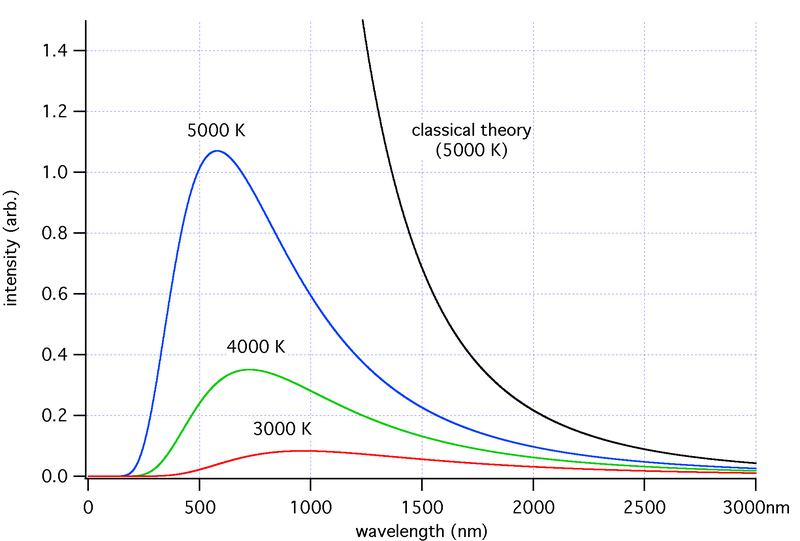
\includegraphics[angle=0,width=0.6\textwidth]{blackbody/planck01.jpg}
		\caption{\label{bb:fig:planck}
			The spectrum of radiation emitted by a perfect blackbody at temperatures of 3000K, 4000K, and 5000K according to the Planck formula is shown by red, green, and blue lines, respectively. The solid black line shows prediction of classical (non-quantum) thermodynamics for emission at 5000K
			%, which is quite different from the Planck formula. It is the Planck formula that describes experimental results and not the classical formula. This discrepancy was one of the
			%main factors that led to development of quantum mechanics that superseded classical theory. 
			(Figure source: Wikipedia.org).}
	\end{center}
\end{figure}

The shape of the blackbody spectrum was measured in laboratory at the end of 19th century and was a source of much puzzlement to the physicists of that time because it contradicted the expectations of classical thermodynamics (the branch of physics studying heat and radiation). Attempts to understand the shape of the blackbody spectrum led to development of quantum mechanics. The formula accurately describing the shape of the measured spectrum was proposed by the German physicist Max Planck in 1900. Planck also showed how this shape can be understood using theoretical calculations based on concepts of quanta of energy and thermodynamic equilibrium. The Planck formula describing the shape of the blackbody spectrum as a function of wavelength $\lambda$ is given by the following formula:

\begin{equation}\label{bb:eq:planck}
B_\lambda (T) = \frac{2 h c^2}{\lambda^5} \frac{1}{\exp(\frac{h c}{\lambda k T}) - 1}
\end{equation}
where $h=6.63\times10^{-34}\,$J/s is the Planck constant, $c=2.99\times 10^8\,$m/s is the speed of light in vacuum, and $k=1.38\times 10^{-23}\,$J/K is the Boltzmann constant.  The Planck spectrum shape for different temperatures along with predictions of the classical theory is shown in Fig.~\ref{bb:fig:planck}.% Note that often the entire spectrum cannot be measured due to limited spectral coverage of equipment. In this case one can measure a portion of the spectrum and still compare it to the blackbody spectrum, as you will see in this lab.

\begin{figure}[htb]
	\begin{center}
		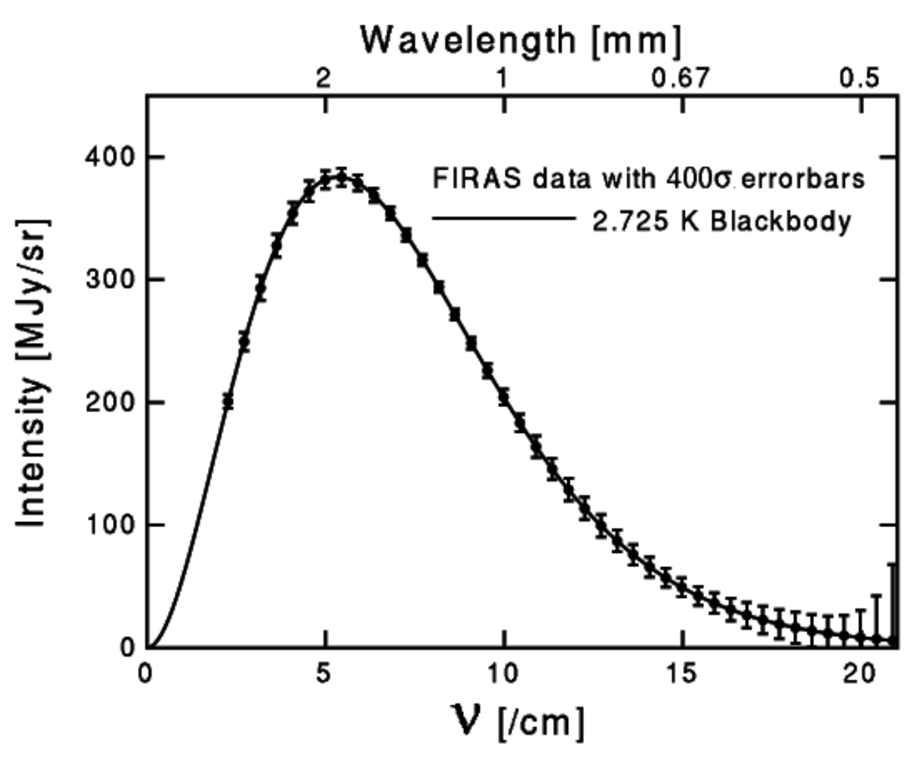
\includegraphics[angle=0,width=0.6\textwidth]{blackbody/firas_spectrum.pdf}
		\caption{Spectrum of CMB as measured by the FIRAS instrument on COBE satellite in the 1990s. Note that the measured spectrum is described almost perfectly by the Planck formula with an effective temperature of 2.7K; the error bars shown are $400 \sigma$!}\label{bb:fig:cobe}
	\end{center}
\end{figure}

Fig.~\ref{bb:fig:cobe} shows the spectrum of the CMB radiation -- a ubiquitous relic radiation from the first few thousand years in the existence of our universe. This radiation was emitted when the universe was very hot and dense and almost in thermodynamic equilibrium. The spectrum is thus very accurately approximated by the Planck formula. %You will measure the CMB radiation and its temperature in one of the labs in PhySci 120 course next quarter. 
Note that this is yet another example of the amazing universality of physical laws in nature. You can use the same formula to describe the spectrum of a regular incandescent bulb and spectrum of relic radiation from the early era of evolution of our universe!

\section{Experimental setup}
\subsection{Spectrometer hardware}

In this lab we will use the the Ocean Optics digital spectrometer, which measures light in the range 350 to 1000 nm with a resolution of about $1\,$nm  ($1\,\textrm{nm} = 10^{-9}\,\textrm{m}$.) Light from the source under study is collected by an optical fiber. \textbf{IMPORTANT: the fiber is fragile, handle with care.} The fiber will be fixed in a holder, which can be adjusted to point to the light bulb. The spectrometer is connected to the computer through USB, and dedicated software (Spectra Suite) is used to operate the spectrometer and save the data. For reference, Fig.~\ref{bb:fig:software1} shows the main controls of the SpectraSuite software.

You will use a regular 25W incandescent light bulb setup in a holder, with a voltage regulator to change the light intensity.

\begin{figure}
	\begin{center}
		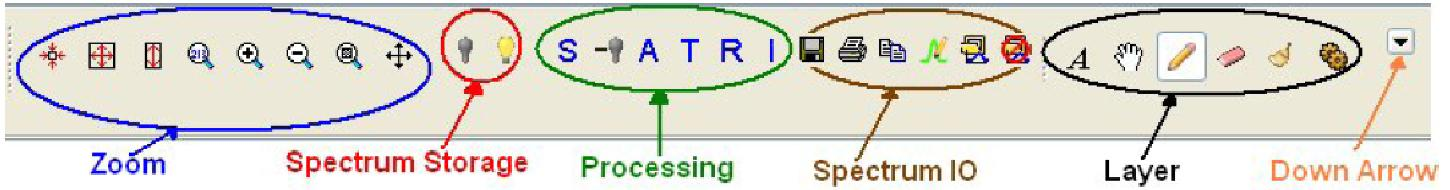
\includegraphics[angle=0,width=1.0\textwidth]{blackbody/software1.jpg}
		\caption{The Spectra Suite software controls: zoom controls can be used to zoom in and
			out the graph. The gray bulb records background (“dark”) spectrum, while the yellow bulb records processed signal spectrum}\label{bb:fig:software1}
	\end{center}
\end{figure}

\subsection{Suggested procedure for saving spectra}
For the following experiments, you can either work alone or in groups of 2. You'll need to operate the voltage control, run the Spectrum Suite software and copy the data and images into Excel and Word documents, and take notes.  Please create a personal folder into which files can be saved, and delete it at the end of the day.

You're welcome to use the software of your choice when completing these assignments; e.g., LibreOffice, Python, or Matlab.  But, in the past most students have found copying and pasting into Word and Excel to be easiest.  To do this, we suggest open a Word and an Excel file in which you save your measured spectra at the beginning of your work.

To save an image of your graph, click on the third from right icon in the Spectrum IO controls (Fig.~\ref{bb:fig:software1}). This will copy image of the graph to the clipboard. Then, paste the image in the Word document by pressing Ctrl-V. To save the spectrum you measured in digital form as two columns of numbers, press the third icon from the left in the Spectrum IO controls (the icon showing two sheets of paper to the right of the printer icon), which will copy the digital spectrum into the clipboard. Now go to an Excel file and choose the column into which you want to paste your spectrum (usually column A, first row) and press Ctrl-V, which will paste the measured spectrum as two columns of numbers (wavelength in nm and counts for your spectrum) into the Excel worksheet.

At the end of the lab, save the Word and Excel files with images of graphs and numerical spectra and their analyses done during the lab on a USB stick or email copies to yourself.  

An alternative, but slower, way to save the data is to click on the floppy disk icon in the Spectrum IO controls. The format must be “Tab delimiter, no header”. The writing directory must be specified (“Browse” button). The spectrum is saved in a text file (.txt) as two columns, the first column giving the wavelength in nm, the second column the corresponding intensity. This file can be imported into an Excel worksheet using Open File within the File menu of Excel.

%\chapter{Behavior of gravity waves in water (the ripple tank)}\label{cha:ripple-tank}

%TODO include theoretical limit considerations in curve fitting

\section{Introduction}

The Michelson interferometer, named after University of Chicago professor Albert A. Michelson (Nobel prize in Physics 1907), is an extremely sensitive instrument capable of measuring incredibly tiny displacements.
A modern version of the Michelson interferometer has been developed by The Laser Interferometer Gravitational-Wave Observatory (LIGO) experiment to detect changes in distance of $10^{-19}\:$m (much less than the size of the nucleus of an atom!).
This displacement is sensed between mirrors separated by 4 km (see Figure~\ref{rt:fig:ligo-aerial}). There are two sites for LIGO --- one in Hanford, WA and the other in Livingston, LA.
The LIGO interferometer has recently detected gravitational waves for the first time (September 15, 2015); the first announced gravitational wave detection fits, with remarkable precision, the expected signal from the merging of two black holes, 29 and 36 solar masses, located 410 Mpc away.
The reported signal and the comparison to the fitted model are shown in Figure~\ref{rt:fig:ligo-signals}.

\begin{figure}
	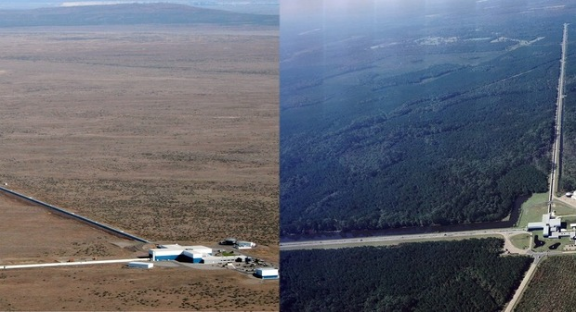
\includegraphics[width=\textwidth]{ripple-tank/ligo-aerial.png}
	\caption{An aerial view of the two LIGO sites.}\label{rt:fig:ligo-aerial}
\end{figure}

\begin{figure}
	\centering
	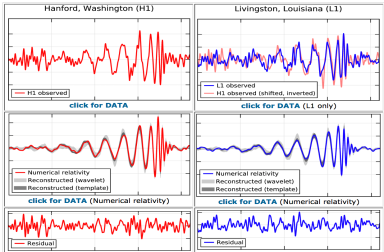
\includegraphics[width=0.7\textwidth]{ripple-tank/ligo-signals.png}
	\caption{The left panels show the LIGO signal at the Hanford site (top) and the best-fit model
		(middle) and the residual of the model minus the data (bottom). The residuals are consistent
		with noise. The right panels show the same for the Livingston site, with the Hanford signal
		plotted in red in the top panel to demonstrate the similarity of the two measurements (as
		expected in the event of a true gravitational wave signal). This first LIGO detection of a
		gravitational wave event marks a significant transformation in our collective ability to
		measure and understand black holes, and since that first detection, more black hole merger
		events have been detected and reported.}\label{rt:fig:ligo-signals}
\end{figure}

The working principle of the Michelson interferometer is the interference of light.
In this lab, you will first explore the concepts of interference with waves produced in water, in a device known as a ripple tank.
In particular, in this first portion of the lab you will experimentally verify a relationship between wave frequency and wavelength, and then demonstrate constructive and destructive wave interference.
You will then extend that understanding of interference to a wave geometry more appropriate to the second portion of the lab.
The final measurement with the ripple tank will allow you to show that plane waves propagating through a slit behave as though the slit were a new source of waves, propagating radially (i.e.\ in a circular pattern).

Next week, you will measure interference phenomena with light, with a modern version of the famous double-slit experiment performed by Thomas Young in 1801.
You will show that the interference properties of waves established in the first section of the lab apply to light as well, thus experimentally demonstrating that light behaves in a wavelike manner.

Having established the wavelike nature of light, you will then finally use a table-top Michelson interferometer to measure changes in distances smaller than a human hair (not quite LIGO sensitivity, but still pretty impressive!).

\section{Learning Goals}

\begin{itemize}
	\item Learn how to conduct an observational experiment, including collecting data and analyzing the data to find and describe a pattern quantitatively.
	
	\item Discover the relationship between frequency and wavelength of waves.
	
	\item Learn how to conduct a testing experiment, including identifying a hypothesis, designing an experiment, making a prediction, and comparing it to an experimental outcome.
	
	\item Gain familiarity with wave interference.
\end{itemize}

\section{An aside: picking a project topic}

By the end of lab today, ensure that you have chosen a topic for your presentation+paper project, and that it has been approved by your TA.

\section{The Scientific Cycle\protect\footnote{adapted from \cite{etkina_college_2014}}}

One way of describing science is the process of incrementally improving a shared model of how our universe works. In different fields of science, different methods and cycles are used, so there is no ``One True Scientific Method.'' One can still create a model for the process of science, and we describe here one such cycle (the hypothetico-deductive cycle), summarized in Figure~\ref{me:fig:isle}.

In this cycle, there are three types of experiments, each one representing a different stage of the scientific effort. One stage, often started when encountering a novel phenomenon, is the \textbf{observational experiment}. This is an experiment that consists of deciding what to observe and how to observe it, collecting data, finding a pattern, and brainstorming possible explanations for what is observed (also called ``hypotheses'').

Once one has some trial explanations, one can test one or more of those with a \textbf{testing experiment}. Here, one designs a new experimental procedure and uses each hypothesis to predict what will happen. Then the prediction is compared to the procedure's outcome. If they are different, then the hypothesis is judged to be not a helpful explanation for that phenomenon. If they are the same, then it is still helpful. Throughout this stage, one may make various assumptions that would need to be validated, as they can effect the prediction or outcome.

Once a hypothesis has been tested enough for people to find it useful, then it can be applied to solve practical problems, or to determine properties of particular situations, in an ``application experiment.''

\begin{figure}
	\centering
	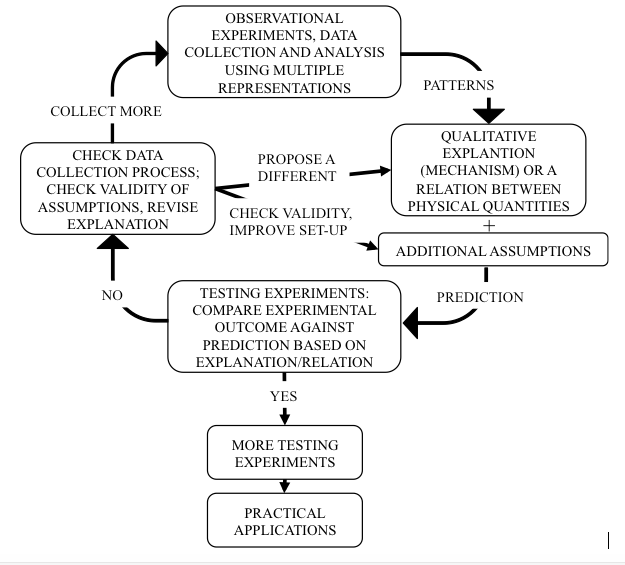
\includegraphics[width=0.7\textwidth]{ripple-tank/islegraphic.png}
	\caption{A model of the process some scientists go through to create knowledge.\cite{etkina_millikan_2015}}\label{me:fig:isle}
\end{figure}

\section{Experiment 1: Observation of frequency and wavelength}

\textbf{Goal:} Observe gravity waves in a ripple tank and determine a mathematical relationship between frequency and wavelength.

\textbf{Available equipment:} ripple tank with strobe light and ripple generator, plane wave attachment, 2 dippers (narrow plastic rods), 1 short wall, 1 medium wall, 2 long walls for ripple tank, flashlights or desk lamps, digital camera (e.g.\ your smartphone), computer with ImageJ installed (can be your device), object of known size to be submerged

\begin{framed}
	\textbf{Caution: Flickering Lights!} You will be using a stroboscopic light in this lab. Such light is known to trigger reactions in some individuals (e.g. photosensitive epilepsy).
	If you are worried that you may be sensitive to strobe light, speak to the TA and skip attending this part of the lab.
	In any case, avoid staring directly at the light.
\end{framed}

\begin{framed}
	\textbf{Self-assessment:} To help you improve your scientific abilities, we provide you with self-assessment rubrics.
	A rubric is a scoring system.
	Self-assessment is determining how well you performed a particular task.
	So, these self-assessment rubrics are designed to help you evaluate your performance while you are designing and performing your experiment.
	
	The complete set of rubrics is available in Appendix~\ref{cha:rubrics}.
	In each lab, your report will be assessed using Rubric F, found in Table~\ref{rubric:f}, as well as 5 additional rubric rows listed in that lab.
	Each week, read through these and use them to evaluate your work as you design and perform the experiment.
	Your instructor will use the same rubrics to determine part of your grade for the lab.
\end{framed}	

\textbf{Rubrics to focus on during this experiment:} B7, B8, F1, F2. See Appendix~\ref{cha:rubrics} for details.

\subsection{The ripple tank and generator}

In this section you will explore interference phenomena using a ripple tank. The tank --- 42.5 cm x 42.5 cm and 2.5
cm deep --- is filled with water, and is equipped with a ripple generator. The generator uses voice coil actuators to
produce the precise and quiet up-and-down motion of the rippler arms. Waves are generated in the tank by the moving
dippers that touch the surface of the water. The generator also controls a light source that produces a bright, clear
image of the wave patterns in the ripple tank. The light can be used as a steady source or as a strobe to ‘freeze’ the
motion of the wave patterns (in this case the flashing light and the generator are driven with the same frequency). The
ripple generator frequency ranges from 1.0 to 50 Hz adjustable in 0.1 Hz increments. You will work with frequencies in
the range 16--32 Hz. A mirror placed below the tank and working in conjunction with a projection screen provide a
magnified image of the wave patterns in the water; you will record patterns seen on this screen by photographing them
with a digital camera. The ripple generator terminates in a bar with numerous clips in which you can place various
``dippers''.

\subsection{Suggestions for your experiment}

\begin{enumerate}
	\item You may want to decide on roles for each group member. Example roles include Facilitator (ensures time and group focus are efficiently used), Scribe (ensures work is recorded), Technician (oversees apparatus assembly, usage), Skeptic (ensures group is questioning itself). Note that each role is responsible for ensuring that the thing happens, rather than necessarily doing it themselves. \textbf{Decide if you are using these roles, and if so, assign them and note them in the lab report.}
	
	\item Ensure that every group member knows what the terms frequency and wavelength mean, in relation to waves. Use whatever means at your disposal to do this.
	
	\item This is an ``observational experiment.'' Review Rubric B (Table~\ref{rubric:b}) and discuss any unclear expectations with your group and the instructor. Note that your lab report will be graded, in part, on demonstration of Abilities B7 and B8.
	
	\item Ensure that one of the ripple tank's ripple generator is set up with 1 dipper fixed in the center clip of the bar that extends from the box, and that the height of the generator is such that the dipper just touches the top of the water. You can make coarse adjustments by moving the generator along the support rod, and fine adjustments with the two red knobs on it.
	
	\item Brainstorm different methods you could use to determine the relationship between wavelength and frequency. Feel free to play with the ripple tank as you do so, seeing what the frequency and amplitude knobs do. Notice that for different frequencies, different amplitudes produce the clearest image. Here are some things to consider:
	\begin{itemize}
		\item Which variable will you control (and thus will be the independent variable) and which will you measure?
		
		\item What is the range of the independent variable that you will use? How many different settings will you choose?
		
		\item You will need to use several settings of the independent variable, and then plot the data in a graph, decide on what pattern you see, and give some justification for that pattern. You can use words like ``proportional'', ``linear'', ``parabolic'', ``exponential'', ``logarithmic'', and so on, if they fit. Ensure you use the mathematical definition of these.
		
		\item How will you measure the wavelength?
		\begin{itemize}
			\item Is it a more precise measurement if you measure several of them at once and divide to get a single wavelength?
			
			\item The reflected image might magnify the ripple tank, so it can be helpful to place an object of known size in the tank, like a coin, so you can determine the correct scaling.
		\end{itemize}
		
		One way to take careful measurements of the wavelength is to take a picture of the projected tank, then use a program like ImageJ to measure the lengths you need. If you do so, one way to keep track of what settings go with what image is to mark a card with the settings and place it in view of the camera. See the section below on measuring lengths with ImageJ.
	\end{itemize}

	\item Decide on your measurement and analysis method and discuss it with an instructor before you begin. They will help increase the chances that your method will lead to successful results, or at least that the unhelpful path that you choose will take a short enough amount of time for you to change it when you discover it does not work. We want you to have productive failure that you have time to learn from.
	
	\item Perform your experiment. Your lab report for this experiment should include:
	\begin{itemize}
		\item A labeled sketch or photo of the setup, and a description of the experimental procedure (see Rubric F1).
		
		\item A plot of wavelength vs. frequency (with the independent variable on the horizontal axis)
		
		\item A description of the pattern found. This can be done with a line (straight or curved) showing the pattern you see (either drawn manually or using the curve fitting function of the plotting program, e.g.\ LibreOffice Calc or Microsoft Excel) and with words describing what you found. (B7)
		
		\item An equation to represent the pattern. This can be taken from a curve fit or found by hand. Make sure there is some discussion of how well the equation agrees with the data, but you don't need to be very precise about it. (B8)
		
		\item A discussion of the findings of the experiment and why it's helpful (for you and/or for science) (F2)
	\end{itemize}

\end{enumerate}

\subsection{Measuring lengths using ImageJ}

ImageJ (\url{http://imagej.nih.gov/ij/download.html}), which is installed on the lab computers, is useful for measuring lengths in images. To do so, load your image, then follow these steps to calibrate the ruler --- that is, to tell ImageJ how long something is in the image, so it knows how many pixels correspond to what length).

\begin{enumerate}
	\item Start with an image that has an object in it that you know one of the lengths of (e.g.\ the length of side, or a diameter).
	
	\item Open that image in ImageJ.
	
	\item Select the icon with the straight line on it, and click and drag along the known length.
	
	\item From the drop-down menu, select ``Analyze'' $>$ ``Set Scale...''.
	
	\item Set ``Known distance'' to the value of the known length.
	
	\item Set ``Unit of length'' to the unit you are using, for example ``mm'' for millimeters.
	
	\item Record the pixel scale given at the bottom of the box for future use.
	
	\item Now when you use the straight line tool, it will give the length in physical units in ImageJ's toolbar.
\end{enumerate}

\section{Experiment 2: Testing the conditions for constructive interference}

\textbf{Goal:} Test the hypothesis that constructive interference between two waves occurs at positions where the distance from each source differs by a half-integer number of wavelengths, or
\begin{equation}
 \Delta d = (m+\frac{1}{2})\lambda \,,
\end{equation}
where $\Delta d$ is the ``path length difference'', $\lambda$ is the wavelength, and $m$ is any integer.

\textbf{Available equation:} Same as in the previous experiment.

\textbf{Setup:} Instead of 1 dipper, use two dippers mounted with 3 empty clips between them on the bar. Ask the TA for assistance in setting this up. Adjust so that the dippers are just resting in the surface of the water. Adjust the frequency and amplitude to get clear, sharp waves.

\textbf{Rubric rows to be assessed in this experiment:} C1, C4, C7, F1, F2. See Appendix~\ref{cha:rubrics} for details.

\subsection{Testing this hypothesis}

In general, one tests a hypothesis by using it to make a prediction about what will happen in a certain experimental procedure. With this hypothesis, it asserts a relationship between path length difference, wavelength, and constructive interference. But there are only certain points on the ripple tank image where it is easy to see constructive interference --- the bright spots at the intersection of waves originating from both sources. For an example, see Figure~\ref{rt:fig:interference-2d}.

\begin{figure}
	\centering
	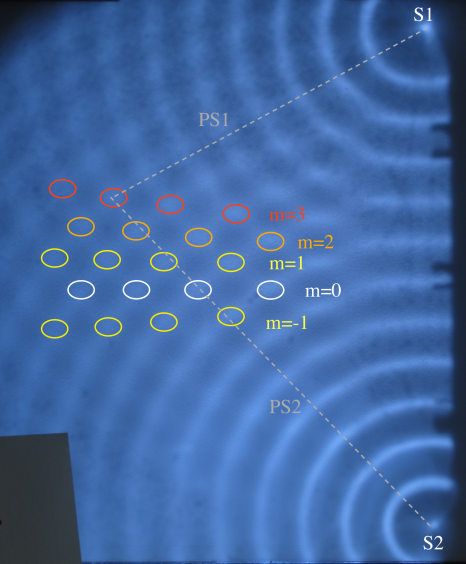
\includegraphics[width=0.7\textwidth]{ripple-tank/interference-2d.png}
	\caption{Example interference pattern for 2 dippers. The bright spots are circled. For a particular bright spot of constructive interference, the two path lengths PS1 and PS2 are drawn.}\label{rt:fig:interference-2d}
\end{figure}

In this case, it is easier to start by finding those locations, measuring the $\Delta d$, finding the wavelength for the given frequency using the relationship you found in Experiment 1, and solving for $m$. The hypothesis predicts that $m$ should always be an integer. As a result, your experiment becomes this: find out how close the experimentally determined $m$'s are to integers.

Brainstorm your experimental procedure, decide on it, discuss with your TA, then perform the experiment.

Your lab report for this experiment should include:
\begin{itemize}
	\item A clear description of the hypothesis (see Rubric C1).
	
	\item A labeled sketch or photo of the setup, and a description of the experimental procedure (F1).
	
	\item A clear statement of the prediction that the hypothesis makes for this particular procedure (C4).

	\item A table of path lengths, path length differences, and measured $m$ values.
	
	\item An analysis of how close the measured $m$ values are to the prediction. Use some quantitative measure of this, but don't worry about being precise about uncertainties (C7).
	
	\item A judgment about the hypothesis. Is it supported, disproved, or undetermined? (C8, though not assessed this time)
	
	\item A discussion of the findings of the experiment and why it's helpful (for you and/or for science) (F2).
\end{itemize}

%In the case of a hypothesis like this one, that includes a proposed equation, there is a useful template for coming up with a prediction:
%\begin{enumerate}
%	\item Note that this hypothesis is asserting that when the equation is true, there is constructive interference (a bright spot). So the goal is to test how true this is.
%	
%	\item Choose which variables you are holding constant, which one is the independent, and which is the dependent variable. In this case, you may not know what $m$ is ahead of time. You could choose it arbitrarily, for example $m=0$ first, and go from there.
%	
%	\item Once you decide on your procedure (which things to measure, how to vary the independent variable), you can use the equation to solve for the dependent variable, which becomes the prediction (Rubric C4).
%	
%	\item The set of dependent variables (for each chosen independent variable) becomes the prediction of the hypothesis that you will use to compare to experimental outcome (C7).
%\end{enumerate}
%
%\subsection{Suggestions for your experiment}
%
%\begin{itemize}
%	\item Note that constructive interference happens where there are bright spots in the projected image at the intersection of waves coming from both sources.
%	
%	\item There is an entire line of points that have the same path length difference from each source, so for each choice of $m$, there can be many 
%\end{itemize}

\section{Experiment 3: Observing plane waves encountering narrow gaps}

This experiment does not clearly follow the model of the scientific cycle, but is closest to an observational experiment. In next week's lab, you will investigate the properties of light traveling through small slits. Ripples in water are more obviously waves, so it is helpful to observe what happens here first.

Instead of dippers, remove them and position the bar so that it is resting in the water. This will produce straight line waves, or, in two dimensions, ``plane waves''. This is the same kind of waves we will use next week with light.

Adjust the amplitude and frequency, with the frequency in the range 20--25 Hz, until you see
clear well-defined vertical parallel lines. Now, insert the two large ``walls'' in the tank, parallel to the rippler bar and
perhaps 5cm away; allow a small (few mm) opening between the two wall sections, placed so that opening is vertically
centered in the projected image. Adjust the amplitude upward until you see a clear wave pattern radiating from that
opening. Take a picture. Repeat this with two apertures instead of one; do this by adding a smaller wall between the
two larger sections, with all sections parallel to the rippler bar, and a small gap between each larger wall and the central
smaller portion. Again, take a picture, adjusting amplitude as necessary to get well-defined waves.

The analysis of this will be done as individual homework.

\section{Individual Homework}

These questions are to be answered individually and your answers should be submitted under the Lab 1 Homework assignment on Canvas.

Both questions concern the last two situations recorded in the lab: the case of 2 walls (1 gap or ``aperture'') and the case with 3 walls (2 apertures).

\begin{enumerate}
	\item What wave pattern do you see in the case of a single aperture? What do you see In the case of a double aperture?
	How do these patterns compare to the data you took using dippers on the rippler bar?
	
	\item Is the wavelength of the pattern you observe consistent with the relationship between frequency and wavelength you
	measured with the dippers? Include any measurements and calculations you make in answering this question in your homework response, and be quantitative.
\end{enumerate}

\appendix

%\chapter{Analysis of Uncertainty}

A physical quantity consists of a value, unit, and uncertainty.
For example, ``$5 \pm 1\,$m'' means that the writer believes the true value of the quantity to most likely lie within 4 and 6 meters\footnote{The phrase ``most likely'' can mean different things depending on who is writing.
	If a physicist gives the value and does not given a further explanation, we can assume that they mean that the measurements are randomly distributed according to a normal distribution around the value given, with a standard deviation of the uncertainty given.
	So if one were to make the same measurement again, the author believes it has a 68\% chance of falling within the range given.
	Disciplines other than physics may intend the uncertainty to be 2 standard deviations.}.
Without knowing the uncertainty of a value, the quantity is next to useless.
For example, in our daily lives, we use an implied uncertainty.
If I say that we should meet at around 5:00 pm, and I arrive at 5:05 pm, you will probably consider that within the range that you would expect.
Perhaps your implied uncertainty is plus or minus 15 minutes.
On the other hand, if I said that we would meet at 5:07 pm, then if I arrive at 5:10 pm, you might be confused, since the implied uncertainty of that time value is more like 1 minute.

Scientists use the mathematics of probability and statistics, along with some intuition, to be precise and clear when talking about uncertainty, and it is vital to understand and report the uncertainty of quantitative results that we present.

\section{Types of measurement uncertainty}

For simplicity, we limit ourselves to the consideration of two types of uncertainty in this lab course, instrumental and random uncertainty.

\subsection{Instrumental uncertainties}

Every measuring instrument has an inherent uncertainty that is determined by the precision	
  of the instrument.
Usually this value is taken as a half of the smallest increment of the instrument's scale. For example, $0.5\:$mm is the precision of a standard metric ruler; $0.5\:$s is the precision of a watch, etc. For electronic digital displays, the equipment's manual often gives the instrument's resolution, which may be larger than that given by the rule above.

Instrumental uncertainties are the easiest ones to estimate, but they are not the only source of the uncertainty in your measured value.
You must be a skillful experimentalist to get rid of all other sources of uncertainty so that all that is left is instrumental uncertainty.

\subsection{Random uncertainties}

Very often when you measure the same physical quantity multiple times, you can get different results each time you measure it.
That happens because different uncontrollable factors affect your results randomly.
This type of uncertainty, random uncertainty, can be estimated only by repeating the same measurement several times.
For example if you measure the distance from a cannon to the place where the fired cannonball hits the ground, you could get different distances every time you repeat the same experiment.	
  
For example, say you took three measurements and obtained 55.7, 49.0, 52.5, 42.4, and 60.2 meters. We can quantify the variation in these measurements by finding their standard deviation using a calculator, spreadsheet, or the formula (assuming the data distributed according to a normal distribution)
\begin{equation}
 \sigma = \sqrt{\sum_{i=1}^{N} \frac{(x_i-\bar{x})^2}{N-1}} \, ,
\end{equation}
where $\{x_1, x_2, \dots, x_N\}$ are the measured values, $\bar{x}$ is the mean of those values, and $N$ is the number of measurements.
For our example, the resulting standard deviation is 6.8 meters. Generally we are interested not in the variation of the measurements themselves, but how uncertain we are of the average of the measurements. The uncertainty of this mean value is given, for a normal distribution, by the so-called ``standard deviation of the mean'', which can be found by dividing the standard deviation by the square root of the number of measurements,
\begin{equation}
\sigma_\textrm{mean} = \frac{\sigma}{\sqrt{N}} \, .
\end{equation}
So, in this example, the uncertainty of the mean is 3.0 meters. We can thus report the length as $52 \pm 3\:$m.

Note that if we take more measurements, the standard deviation of those measurements will not generally change, since the variability of our measurements shouldn't change over time. However, the standard deviation of the mean, and thus the uncertainty, will decrease.

\section{Propagation of uncertainty}

When we use an uncertain quantity in a calculation, the result is also uncertain. To determine by how much, we give some simple rules for basic calculations, and then a more general rule for use with any calculation which requires knowledge of calculus. Note that these rules are strictly valid only for values that are normally distributed, though for the purpose of this course, we will use these formulas regardless of the underlying distributions, unless otherwise stated, for simplicity.

If the measurements are completely independent of each other, then for quantities $a \pm \delta a$ and $b \pm \delta b$, we can use the following formulas:
\begin{equation}\label{unc:add}
\textrm{For } c = a + b \textrm{ (or for subtraction), } \delta c = \sqrt{(\delta a)^2 + (\delta b)^2}
\end{equation}

\begin{equation}\label{unc:mult}
\textrm{For } c = ab \textrm{ (or for division), } \frac{\delta c}{c} = \sqrt{\left(\frac{\delta a}{a}\right)^2 + \left(\frac{\delta b}{b}\right)^2}
\end{equation}

\begin{equation}\label{unc:exp}
\textrm{For } c = a^n,\, \frac{\delta c}{c} = n \frac{\delta a}{a}
\end{equation}

If you are familiar with calculus, you may want to use this general formula for the uncertainty $\delta f$ of a function $f$ of $N$ independent values $x_i$, each with uncertainty $\delta x_i$:
\begin{equation}\label{unc:general}
\delta f = \sqrt{ \sum_{i=1}^{N} \left(\frac{\partial f}{\partial x_i} \delta x_i\right)^2 } \, .
\end{equation}
Notice that Eqs.\ \ref{unc:add} through \ref{unc:exp} can be derived from Eq.\ \ref{unc:general} for those specific cases.

\subsubsection{What if there is no reported uncertainty?}

Sometimes you'll be calculating with numbers that have no uncertainty given.
In some cases, the number is exact.
For example, the circumference $C$ of a circle is given by $C = 2 \pi r$. Here, the coefficient, $2\pi$, is an exact quantity and you can treat its uncertainty as zero.
If you find a value that you think is uncertain, but the uncertainty is not given, a good rule of thumb is to assume that the uncertainty is half the right-most significant digit.
So if you are given a measured length of $1400\:$m, then you might assume that the uncertainty is $50\:$m.
This is an assumption, however, and should be described as such in your lab report.
For more examples, see Table~\ref{unc:tab:implied}.

\begin{table}
	\begin{center}
		\begin{tabular}{cc}
			\textbf{Expression} & \textbf{Implied uncertainty} \\
			12 & 0.5 \\
			12.0 & 0.05 \\
			120 & 5 \\
			120. & 0.5
		\end{tabular}
		\caption{Expression of numbers and their implied uncertainty.}\label{unc:tab:implied}
	\end{center}
\end{table}

\subsubsection{How many digits to report?}

After even a single calculation, a calculator will often give ten or more digits in an answer.
For example, if I travel $11.3 \pm 0.1\:$km in $350 \pm 10\:$s, then my average speed will be the distance divided by the duration. Entering this into my calculator, I get the resulting value ``\texttt{0.0322857142857143}''.
Perhaps it is obvious that my distance and duration measurements were not precise enough for all of those digits to be useful information.
We can use the propagated uncertainty to decide how many decimals to include.
Using the formulas above, I find that the uncertainty in the speed is given by my calculator as ``\texttt{9.65683578099600e-04}'', where the `\texttt{e}' stands for ``times ten to the''.
I definitely do not know my uncertainty to 14 decimal places.
For reporting uncertainties, it general suffices to use just the 1 or 2 left-most significant digits, unless you have a more sophisticated method of quantifying your uncertainties.
So here, I would round this to 1 significant digit, resulting in an uncertainty of $0.001\:$km/s.
Now I have a guide for how many digits to report in my value.
Any decimal places to the right of the one given in the uncertainty are distinctly unhelpful, so I report my average speed as ``$0.032 \pm 0.001\:$km/s''.
You may also see the equivalent, more succinct notation ``$0.032(1)\:$km/s''.

\section{Comparing two values}\label{unc:sec:comparing}

If we compare two quantities and want to find out how different they are from each other, we can use a measure we call a $t'$ value (pronounced ``tee prime''). This measure is not a standard statistical measure, but it is simple and its meaning is clear for us.

Operationally, for two quantities having the same unit, $a \pm \delta a$ and $b \pm \delta b$, the measure is defined as\footnote{Statistically, if $\delta a$ and $\delta b$ are uncorrelated, random uncertainties, then $t'$ represents how many standard deviations the difference $a - b$ is away from zero.}

\begin{equation}
%t' = \frac{\abs{a-b}}{\sqrt{(\delta a)^2 + (\delta b)^2}}
t' = \frac{\abs{a-b}}{\sqrt{(\delta a)^2 + (\delta b)^2}}
\end{equation}

If $t' \lesssim 1$, then the values are so close to each other that they are indistinguishable. It is either that they represent the same true value, or that the measurement should be improved to reduce the uncertainty.

If $1 \lesssim t' \lesssim 3$, then the result is inconclusive. One should improve the experiment to reduce the uncertainty.

If $t' \gtrsim 3$, then the true values are very probably different from each other.
%\begin{landscape}
\chapter{Rubrics}
	
	\freetabcaption{Rubric B: Ability to design and conduct an observational experiment \cite{etkina_scientific_2006}.}
	\begin{longtable}{>{\bfseries}p{0.02\textheight}|>{\bfseries\RaggedRight}p{0.25\textheight}|>{\RaggedRight}p{0.21\textheight}|>{\RaggedRight}p{0.21\textheight}|>{\RaggedRight}p{0.22\textheight}|>{\RaggedRight}p{0.22\textheight}}
		\toprule
		& Scientific Ability
		& Missing & Inadequate & Needs Improvement & Adequate \\ \midrule \endhead
		B1
		& Is able to identify the phenomenon to be investigated
		& No phenomenon is mentioned
		& The description of the phenomenon to be investigated is confusing, or it is not the phenomenon of interest.
		& \midsloppy The description of the phenomenon is vague or incomplete.
		& The phenomenon to be investigated is clearly stated. \\ \midrule
		B2
		& Is able to design a reliable experiment that investigates the phenomenon
		& The experiment does not investigate the phenomenon.
		& The experiment may not yield any interesting patterns.
		& Some important aspects of the phenomenon will not be observable.
		& The experiment might yield interesting patterns relevant to the investigation of the phenomenon. \\ \midrule
		B3
		& Is able to decide what physical quantities are to be measured and identify independent and dependent variables
		& The physical quantities are irrelevant.
		& Only some of physical quantities are relevant.
		& The physical quantities are relevant. However, independent and dependent variables are not identified.
		& The physical quantities are relevant and independent and dependent variables are identified. \\ \midrule
		B4
		& Is able to describe how to use available equipment to make measurements
		& At least one of the chosen measurements cannot be made with the available equipment.
		& All chosen measurements can be made, but no details are given about how it is done.
		& All chosen measurements can be made, but the details of how it is done are vague or incomplete.
		& All chosen measurements can be made and all details of how it is done are clearly provided. \\ \midrule
		B5
		& Is able to describe what is observed without trying to explain, both in words and by means of a picture of the experimental setup.
		& No description is mentioned.
		& A description is incomplete. No labeled sketch is present. Or, observations are adjusted to fit expectations.
		& A description is complete, but mixed up with explanations or pattern. Or the sketch is present but is difficult to understand.
		& Clearly describes what happens in the experiments both verbally and with a sketch. Provides other representations when necessary (tables and graphs). \\ \midrule
		B6
		& Is able to identify the shortcomings in an experiment and suggest improvements
		& No attempt is made to identify any shortcomings of the experiment.
		& The shortcomings are described vaguely and no suggestions for improvement are made.
		& Not all aspects of the design are considered in terms of shortcomings or improvements.
		& All major shortcomings of the experiment are identified and reasonable suggestions for improvement are made. \\ \midrule
		B7
		& Is able to identify a pattern in the data
		& No attempt is made to search for a pattern.
		& The pattern described is irrelevant or inconsistent with the data.
		& The pattern has minor errors or omissions. Terms like ``proportional'' used without clarity, e.g.\ is the proportionality linear, quadratic, etc.
		& The pattern represents the relevant trend in the data. When possible, the trend is described in words. \\ \midrule
		B8
		& Is able to represent a pattern mathematically (if applicable)
		& No attempt is made to represent a pattern mathematically.
		& The mathematical expression does not represent the trend.
		& No analysis of how well the expression agrees with the data is included, or some features of the pattern are missing.
		& The expression represents the trend completely and an analysis of how well it agrees with the data is included. \\ \midrule
		B9
		& Is able to devise an explanation for an observed pattern
		& No attempt is made to explain the observed pattern.
		& An explanation is vague, not testable, or contradicts the pattern.
		& An explanation contradicts previous knowledge or the reasoning is flawed.
		& A reasonable explanation is made. It is testable and it explains the observed pattern. \\
		\bottomrule
	\end{longtable}

	
%\end{table}

\end{landscape}
\chapter{Lab Report Format}

Following the last session of a particular lab, each person will be responsible for turning in a lab report. In a general sense, the labs should demonstrate Rubric Rows F1 and F2 (see Table~\ref{rubric:f}), in addition to the other rubric rows listed in the lab write-up.

\section{General}

\begin{itemize}
	\item The report should be typed for ease of reading. Text should be double-spaced, and the page margins (including headers and footers) should be approximately $2.5\:$cm, for ease of marking by the grader. Each page should be numbered.
	
	\item The first page should include the title of the lab; lab section day, time, and number; and the names of the other members of your lab team.
	
	\item If the rubric row refers to a particular part of your lab report, clearly label that part of the report with that rubric row. For example, you should label the section where you demonstrate uncertainty propagation with ``G2'' if that rubric row is being assessed in that lab.
\end{itemize}

\section{Organizing the report}

If the lab is clearly framed as an observational, testing, or application experiment, you can follow the corresponding rubric for the elements to include in the report (see, respectively, Rubrics B, C, and D in Appendix~\ref{cha:rubrics}).

In general, the report \textbf{must} include the following sections:
\begin{enumerate}
	\item \textbf{Introduction.} A written description of what the lab is designed to investigate and a brief summary of the procedure used. This section should be at least a full paragraph long, and not more than 3 double-space pages.
	
	You don't need to include too much detail here, but it should be a complete and concise description of the purpose and general method used in the lab. Imagine a classmate who hasn't seen the lab writeup asked you, ``what is this lab about? What do you do?'' You should be able to hand them your introduction, and they'd be able to understand the purpose and general structure of the lab. But you need not mention every step and calculation here.
	
	\item \textbf{Analysis and discussion.} For most labs that have more than one part, this should be broken up into parts and labeled in order. This section must include all of the following, in the same order in which these elements appear in the lab instructions.
	\begin{itemize}
		\item Any data that you've collected: tables, figures, measured values, sketches. Whenever possible, include an estimate of the uncertainty of measured values.
		
		\item Any calculations that you perform using your data, and the final results of your calculation. Note that you must show your work in order to demonstrate to the grader that you have actually done it. Even if you're just plugging numbers into an equation, you should write down the equation and all the values that go into it. This includes calculating uncertainty and propagation of uncertainty.
		
		\item If you are using software to perform a calculation, you should explicitly record what you've done. For example, ``Using Excel we fit a straight line to the velocity vs. time graph. The resulting equation is $v = (0.92\:\mathrm{m/s^2}) t + 0.2\:\mathrm{m/s}$.
		
		\item Answers to any questions that appear in the lab handout.
	\end{itemize}

	\item \textbf{Conclusion.} This can be very short, and will generally only require one or two paragraphs. In your conclusion, you should summarize the point of the lab and what you learned, both in the frame of a scientist conducting the experiment (``What did the experiment tell us about the world?'') and in the frame of a student (``What skills or mindsets did I learn?'').
\end{enumerate}

\section{Graphs, Tables, and Figures}

Any graph, table, or figure (a figure is any graphic, for example a sketch) should include a caption describing what it is about and what features are important, or any helpful orientation to it. The reader should be able to understand the basics of what a graph, table, or figure is saying and why it is important without referring to the text. For more examples, see any such element in this lab manual.

Each of these elements has some particular conventions.

\subsection{Tables}

A table is a way to represent tabular data in a quantitative, precise form. Each column in the table should have a heading that describes the quantity name and the unit abbreviation in parentheses. For example, if you are reporting distance in parsecs, then the column heading should be something like ``distance (pc)''. This way, when reporting the distance itself in the column, you do not need to list the unit with every number.

\subsection{Graphs}

A graph is a visual way of representing data. It is helpful for communicating a visual summary of the data and any patterns that are found.

The following are necessary elements of a graph of two-dimensional data (for example, distance vs. time, or current vs. voltage) presented in a scatter plot.

\begin{itemize}
	\item \textbf{Proper axes.} The conventional way of reading a graph is to see how the variable on the vertical axis changes when the variable on the horizontal axis changes. If there are independent and dependent variables, then the independent variable should be along the horizontal axis.
	
	\item \textbf{Axis labels.} The axes should each be labeled with the quantity name and the unit abbreviation in parentheses. For example, if you are plotting distance in parsecs, then the axis label should be something like ``distance (pc)''.
	
	\item \textbf{Uncertainty bars.} If any quantities have an uncertainty, then these should be represented with so-called ``error bars'', along both axes if present. If the uncertainties are smaller than the symbol used for the data points, then this should be explained in the caption.

\end{itemize}

%\chapter{Manual: PASCO Cavendish Balance}\label{cha:pasco-cavendish}

On the following pages is the manual for the PASCO Cavendish Balance.

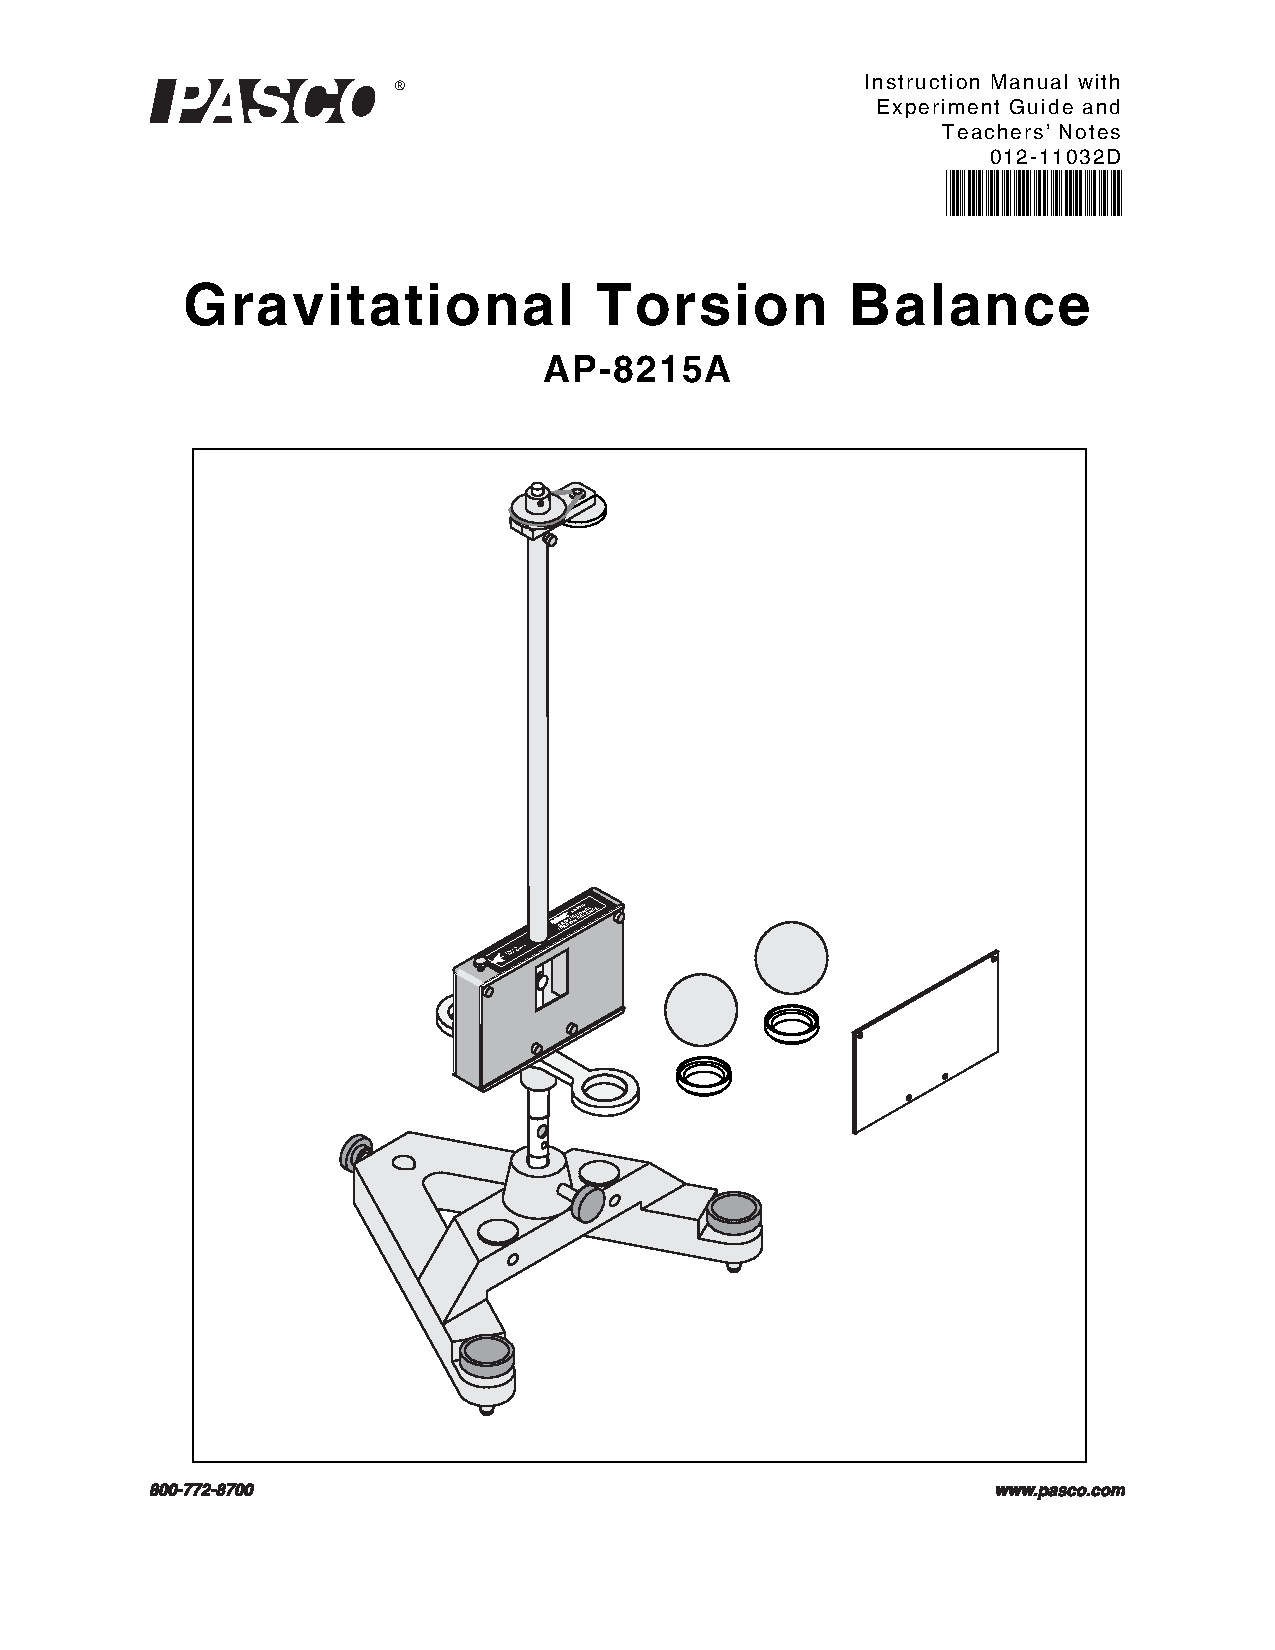
\includepdf[pages={1,3-8,16}]{pasco-cavendish/Gravitational-Torsion-Balance-Manual-AP-8215A.pdf}

% \bibliography{references,MyLibrary}
% \bibliographystyle{plain}
\printbibliography

\end{document}
